
%(BEGIN_QUESTION)
% Copyright 2015, Tony R. Kuphaldt, released under the Creative Commons Attribution License (v 1.0)
% This means you may do almost anything with this work of mine, so long as you give me proper credit

A {\it tachogenerator} is a small DC generator designed to output a voltage directly proportional to the speed of a rotating shaft.  These instruments are used to generate an analog electrical signal representing the rotary speed of a mechanism.  An {\it indicator} is an instrument used to display a measured variable to a human.  A {\it recorder} is a similar instrument used to display a measured variable as a ``trend'' graph over time.  A {\it Data Acquisition Unit} (abbreviated {\it DAQ}) inputs one or more analog electrical signal and outputs a digital number representing those signals, essentially a set of analog-to-digital converters combined with digital networking circuitry.  DAQ units are often used in {\it telemetry} systems where various measurements must be taken and reported over long distances via a digital network such as Ethernet or radio.

\vskip 10pt

With these definitions in mind, examine the following pictorial diagram and explain the purpose of each component within the system:

$$\includegraphics[width=15.5cm]{i03867x01.eps}$$

Suppose the diesel engine happens to be running at full speed (2000 revolutions per minute, or 2000 {\it RPM}).  Identify the amount of voltage we would expect to measure between the following pairs of points in the circuit at this engine speed:

\begin{itemize}
\item{} $V_{21-24}$ = \underbar{\hskip 50pt} volts
\vskip 5pt
\item{} $V_{22-COM}$ = \underbar{\hskip 50pt} volts
\vskip 5pt
\item{} $V_{24-COM}$ = \underbar{\hskip 50pt} volts
\end{itemize}

\underbar{file i03867}
%(END_QUESTION)





%(BEGIN_ANSWER)


%(END_ANSWER)





%(BEGIN_NOTES)

The indicator is simply a DC voltmeter with a scale that reads 0 to 2000 RPM, driven directly by the 0-10 volt signal produced by the tachogenerator.

\vskip 10pt

The three resistors on the terminal block comprise a voltage divider to take the tachogenerator's 0-10 volt signal and reduce it to 0-2 volts DC for the DAQ to measure.

\vskip 10pt

The DAQ is a multi-channel voltage-sensing analog-to-digital converter.  In this system we are only using channel 2 of the DAQ to sense engine speed.

\vskip 10pt

The computer monitor communicates with the DAQ via an Ethernet network, displaying engine speed (represented by the DAQ's sensed voltage signal on channel 2) as a trend graph over time.

\begin{itemize}
\item{} $V_{21-24}$ = \underbar{\bf 10} volts
\vskip 5pt
\item{} $V_{22-COM}$ = \underbar{\bf 6} volts
\vskip 5pt
\item{} $V_{24-COM}$ = \underbar{\bf 0} volts (these are equipotential points)
\end{itemize}

%INDEX% Pictorial circuit review (analog signal wiring to data acquisition unit)

%(END_NOTES)


